%-------------------------------------------------------------------------------
\chapter[Introduction]{Introduction to Sisyphe}
%-------------------------------------------------------------------------------

%-------------------------------------------------------------------------------
\section{Preliminaries}
%-------------------------------------------------------------------------------
\sisyphe{} is the open-source, sediment transport and bed evolution module of the \telemacsystem{}. This module can be used to model complex morphodynamics processes in diverse environments, such as
coastal, rivers, lakes and estuaries, for different flow states, sediment size classes and sediment
transport modes.

In \sisyphe{}, sediment transport processes are grouped as bedload, suspended load or total load,
with an extensive library of predictors for sediment carrying capacity. It is applicable to non-cohesive sediments that can be uniform (single-sized) or non-uniform
(graded), cohesive sediments, as well as sand-mud
mixtures.

A number of physically-based processes are incorporated into \sisyphe{}, such as the influence of
secondary currents to precisely capture the complex flow field induced by channel curvature, the
effect of bed slope associated with the influence of gravity, bed roughness predictors, and areas of
non-erodible bed, among others.

For currents only, \sisyphe{} can be coupled to the depth-averaged shallow water module
\telemac{2D} or to the three-dimensional Reynolds-averaged Navier-Stokes module \telemac{3D}.
To account for the effect of waves or combined waves and currents, \sisyphe can be internally coupled
to the waves module \tomawac{}.

\sisyphe{} can easily be expanded and customized to particular requirements by modifying friendly,
easy to read fortran files. An overview of different applications of \sisyphe{} can be consulted in the yearly-published Telemac-Mascaret User Conference proceedings, freely available at \texttt{www.opentelemac.org}.

\begin{figure}[H]%
\begin{center}
%
\hfil
%
\subfloat[Bar formation and propagation in straight channels: simulations by \sisyphe{} coupled to \telemac{2D} (based on the works by Defina~\cite{Defina2003} and Crosato et al.~\cite{Crosato2011})]{
%
  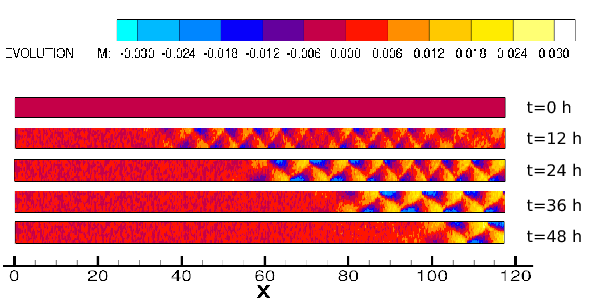
\includegraphics[width=0.5\textwidth]{./graphics/T2d+Sis_Lanzoni_random_10mm_Planimetric.png}
%
}
%
\hfil
%
\subfloat[Point bars in large-amplitude meanders: simulations by \sisyphe{} coupled to \telemac{2D} and \telemac{3D} (based on the experiences by Whiting and Dietrich~\cite{Whiting1993a, Whiting1993b}.]{
%
  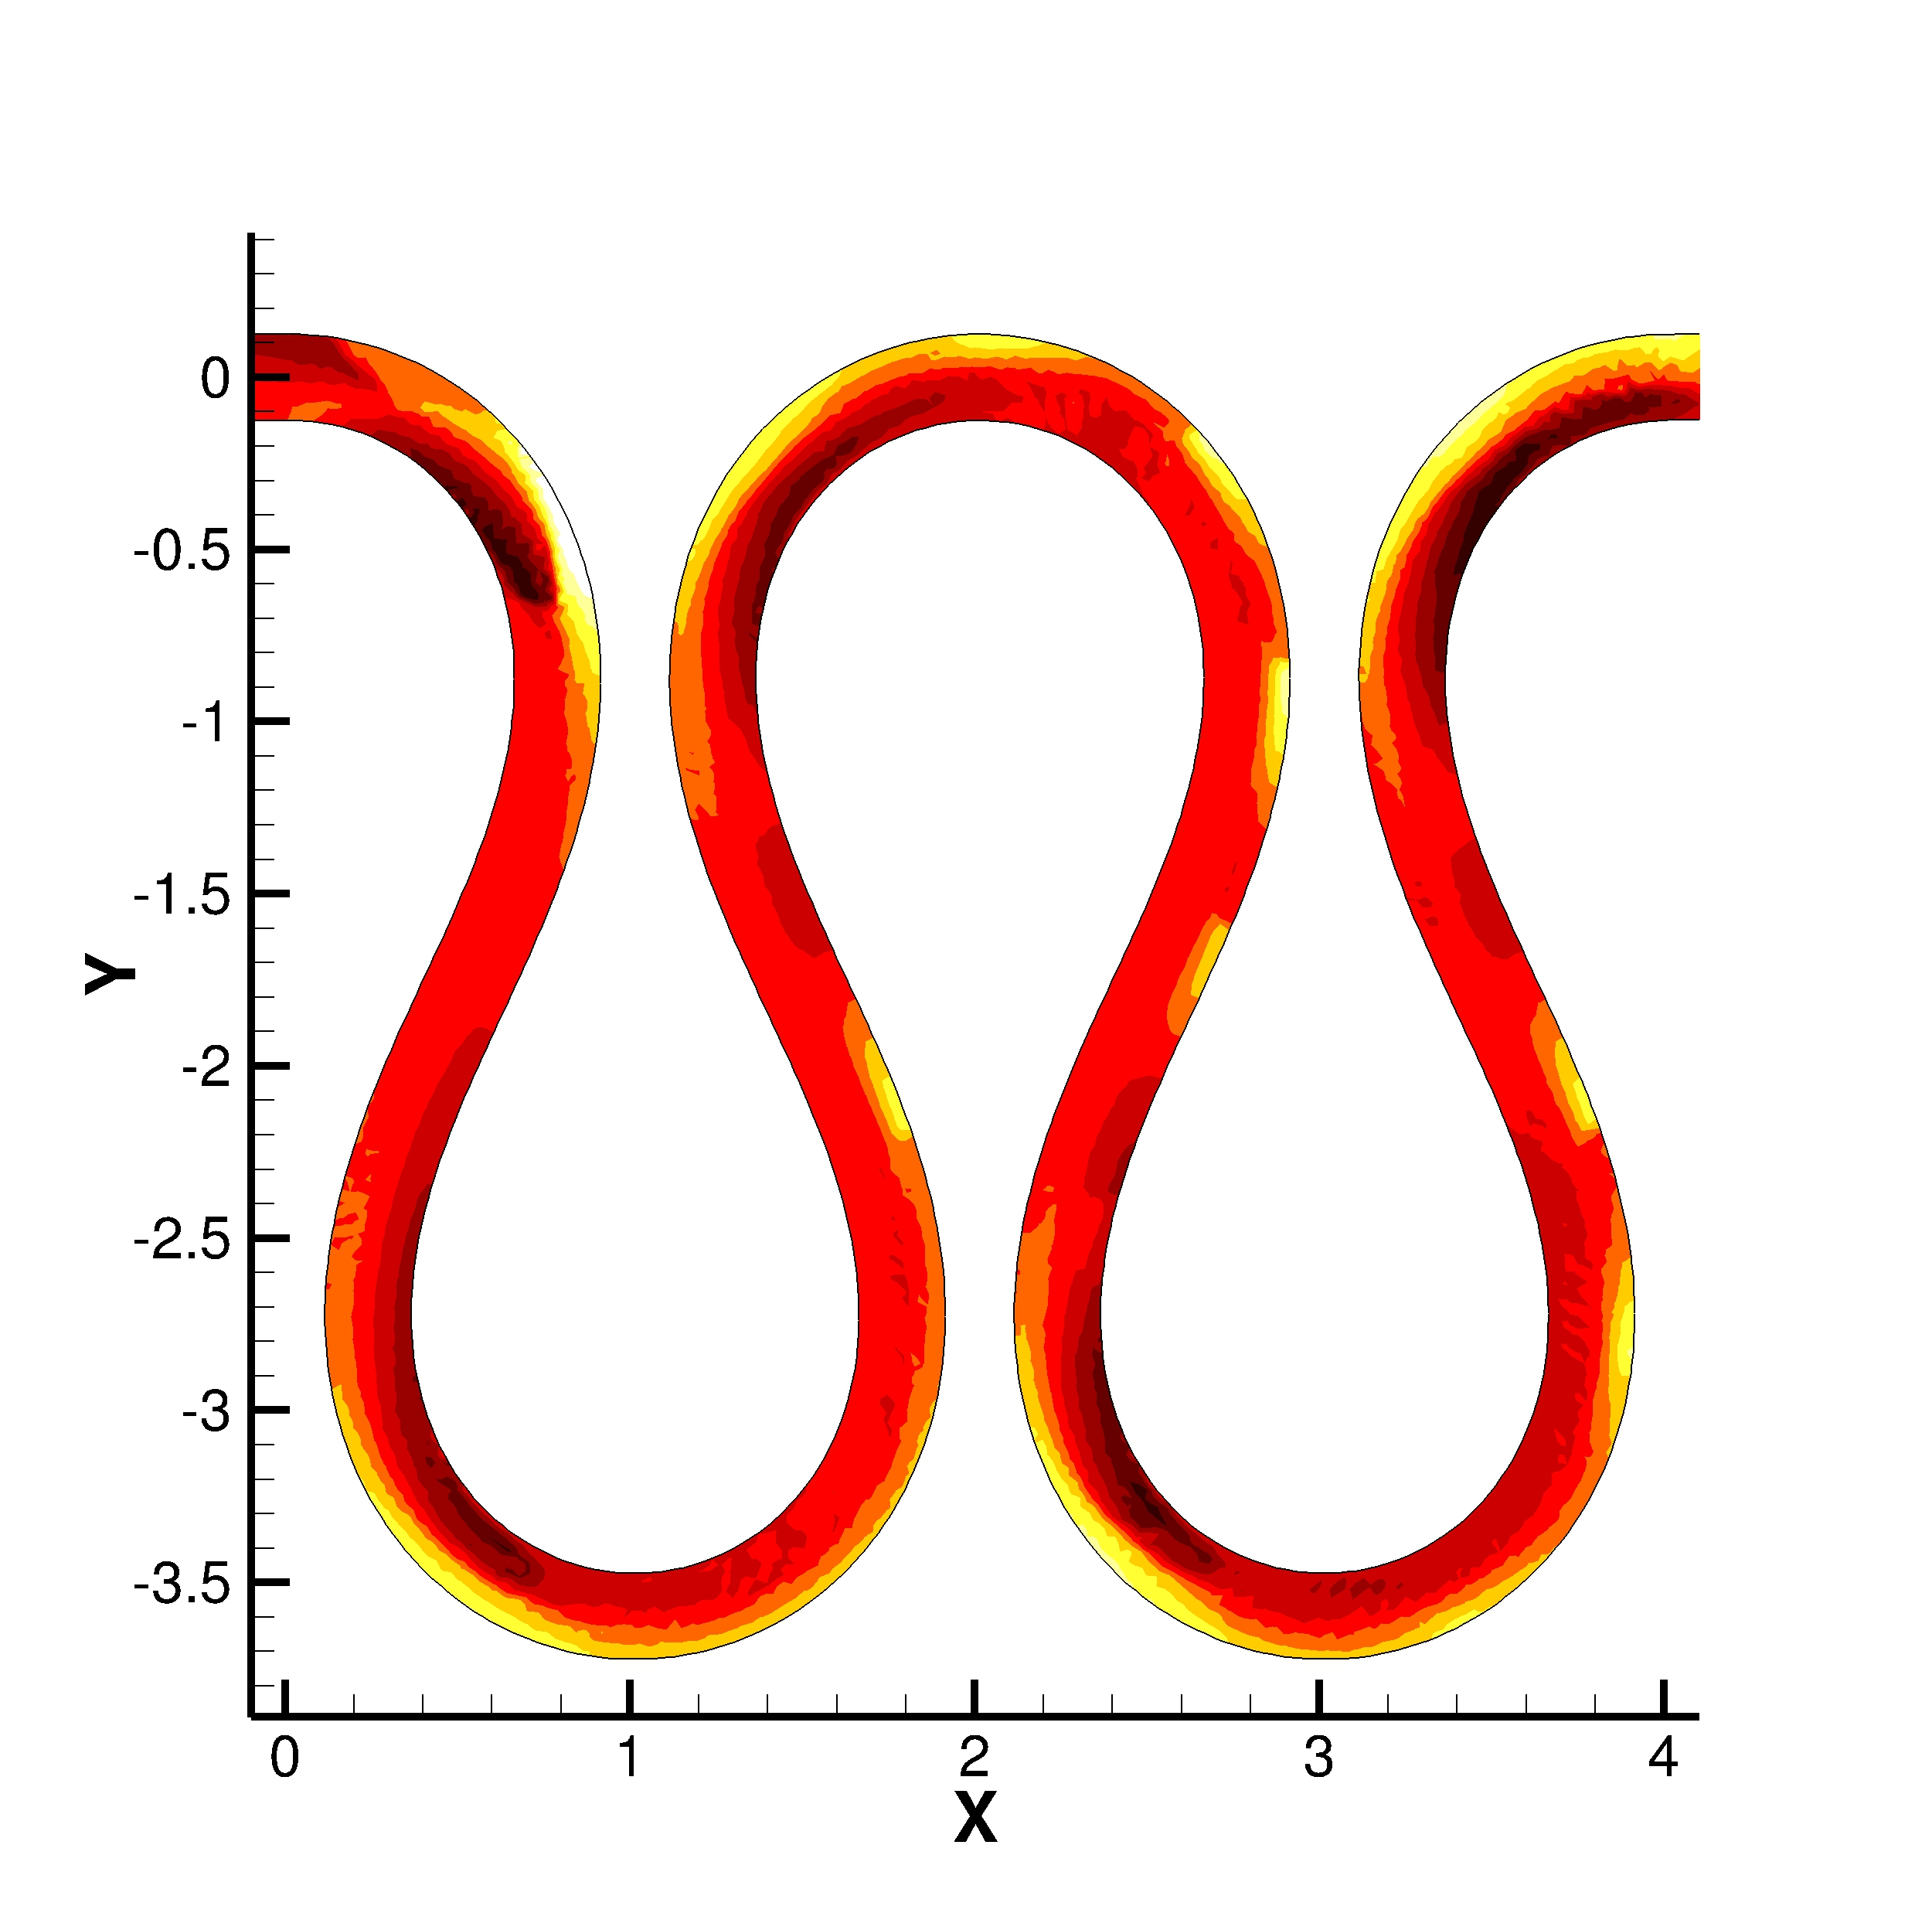
\includegraphics[width=0.35\textwidth]{./graphics/2D.jpg}
%
}

%
\hfil
\mbox{}
\end{center}
\caption
[Examples of morphodynamics modelling]
{Examples of morphodynamics modelling of bar formation and propagation in straight and curved channels. See also proceedings of the Telemac-Mascaret User Conference 2013.}
\label{fig:ExampleMultipleImages}
\end{figure}

%-------------------------------------------------------------------------------
\subsection{Morphodynamic modelling}
%-------------------------------------------------------------------------------
The prediction of topography changes and sediment discharges can be performed by {\bf integrating in a mathematical model}
several modules. It is a {\bf multi--scale problem}, with different physical mechanisms acting according to their space and time response. In summary, the relevant
mechanisms that drives morphological changes are:
\begin{itemize}
         \item {\bf Hydrodynamics}, with conservative laws of mass and momentum 
         \item {\bf Sediment transport}, with predictors for sediment carrying capacity 
         \item {\bf Bed evolution}, with conservative law for sediment mass 
\end{itemize}
\noindent
Such a modelling system is often referred to as a \emph{morphodynamic model} and is the one adopted in the \telemacsystem{}.

\noindent
From the literature, the mechanisms of transport are mainly classified as:
\begin{itemize}
\item \textcolor{black}{\bf bedload:} with a variety of sediment transport parameterizations
\item \textcolor{black}{\bf suspended load:} with the solution of the advection-diffusion equation (ADE) plus closures for erosion and deposition fluxes, equilibrium concentration
\item \textcolor{black}{\bf bed evolution:} with the solution of the sediment mass conservation equation or \textit{Exner equation}.
\end{itemize}

\noindent
Different types of sediment can be classified as:
\begin{itemize}
\item \textcolor{black}{\bf non-cohesive:} equilibrium formulas
\item \textcolor{black}{\bf cohesive:} erosion and deposition laws, consolidation models
\item \textcolor{black}{\bf mixed-size sediments:} moderately/poorly sorted sediment distribution, sand-gravel and sand-mud mixtures
\end{itemize}
\noindent


%-------------------------------------------------------------------------------
\subsection{Two-dimensional morphodynamics modelling with Telemac Modelling System}
%-------------------------------------------------------------------------------
The choice of appropriate model equations for flow and sediment transport
will depend upon the scales of interest. 

At the scale of ripples, the mechanics of sediment transport could be coupled with the
Reynolds--averaged Navier Stokes equations (NS) to describe the phenomenon.
At large scales, however, the shallow water equations (SWE) are known to
capture quite accurately the salient features --in an average sense-- of 
open channel flows. The SWE are derived by simplifying the hydrodynamics in the vertical
direction instead of using the full three--dimensional NS or Euler
equations.

As such, the SWE are obtained by assuming a hydrostatic pressure
distribution and a uniform velocity profile across the water layer,
resulting in a two--dimensional problem where the primary variables are the
vertical averages of the horizontal fluid velocities and the fluid depth.

This simplification enhances the speed of computations and
facilitates further analytical approaches. In brief, the SWE are often
used to model advection--dominated open channel flows, river and lake
hydrodynamics, floodplain flows, estuarine and coastal circulation as well
as long wave run-up and hydraulic bores, among
other problems of interest within the engineering community~\cite{Vreugdenhil:94}. 

\sisyphe{} can be coupled with the SWE solver \telemac{2D} and the NS solver \telemac{3D} (see \S\ref{ch:3DBedloadTransport}). 

%-------------------------------------------------------------------------------
\subsection{Morphodynamics coupling}
%-------------------------------------------------------------------------------
Morphological models can be fully coupled~\cite{cao02} and decoupled~\cite{vriend87}. In a fully coupled model, sediment
transport and flow occur simultaneously, and thus, their respective
equations are coupled and should be solved simultaneously. Rapid morphological evolution processes due
to hyper-concentrated sediment--laden floods, and debris flow are typical
examples were the fully coupled approach must be employed~\cite{Frac02}.

In contrast, decoupled models are applicable when the typical time scale for river or sea bed adjustment 
is much longer than the typical time scale for water flow. The approach used by \sisyphe{} follows the decoupled treatment, i.e., to alternate between the simulation of flow and bed evolution. This procedure, also known as \textit{asynchronous} solution, considers that the bottom is fixed when the flow variables are computed.

Hydrodynamic solution is therefore to solve the hydrodynamic continuity and momentum equations on the fast time scale. The discretization of bottom is then fixed on the fast time scale,
and the discretized sediment equation is subsequently solved separately.


\begin{figure}[H]%
\begin{center}
%
\hfil
%
\subfloat[currents only]{
  %
  \vspace{-1cm}
  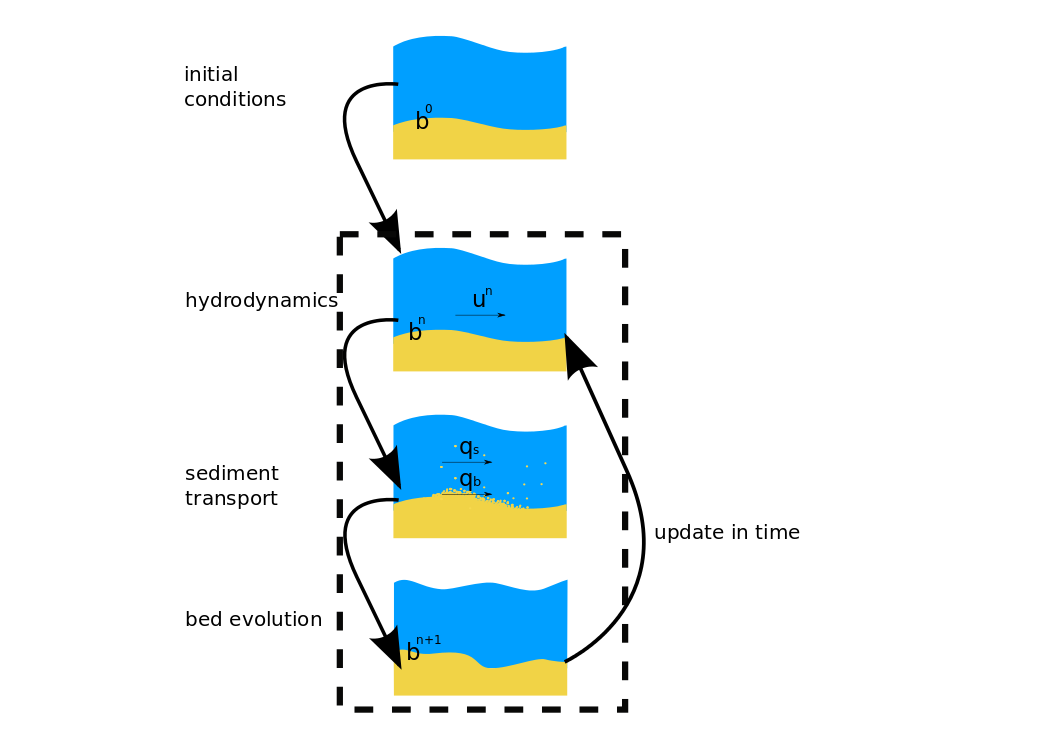
\includegraphics[width=0.55\textwidth]{./graphics/2waycoupling.png}
%
}
%
\hfil
%
\subfloat[currents $+$ waves]{
%
  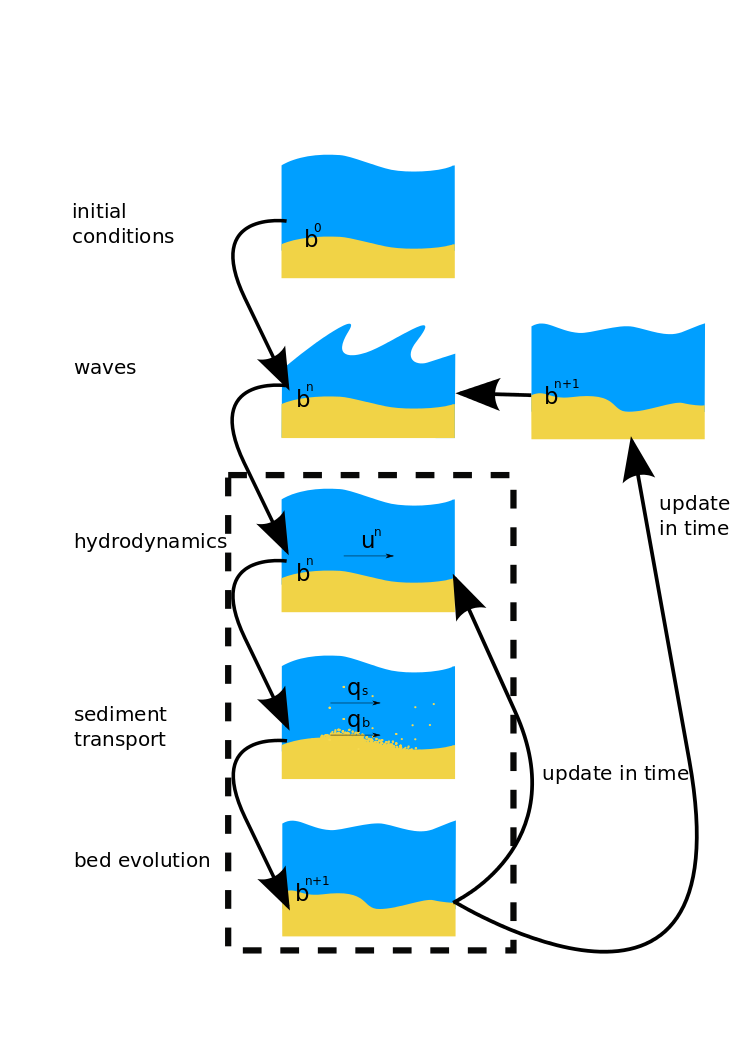
\includegraphics[width=0.4\textwidth]{./graphics/3waycoupling.png}
%
}
%
\hfil
\mbox{}
\end{center}
\caption
[Coupling strategies]
{Schematic coupling strategies for \sisyphe: (a) coupling morphodynamique ``classique'', (b) coupling morphodynamique including the effect of waves.}
\label{fig:CouplingStrategies}
\end{figure}

\pagebreak

%...............................................................................
\section{Running a morphodynamics simulation: first steps}
%...............................................................................
The minimum set of files to run a morphodynamics simulation includes:
\begin{itemize}
\item the steering file (text/ascii file \texttt{*.cas})
\item the geometry file (format selafin/binary \texttt{*.slf})
\item the boundary conditions file (text/ascii file \texttt{*.cli})
\item additional or optional input files as the fortran file (text/ascii file \texttt{*.f}), the reference file (format selafin/binary \texttt{*.slf}), etc.
\end{itemize}

Typically, these files are contained in a folder, for example in the folder {\texttt simulation\}:
\begin{footnotesize}
\begin{verbatim}
simulation\bc_bifurcation_tel.cli
simulation\geo_bifurcation.slf
simulation\res_bifurcation_hotstart_tel.slf  
simulation\run_bifurcation_sis.cas
simulation\run_bifurcation_tel.cas
\end{verbatim}
\end{footnotesize}

Running a simulation from a Linux terminal:
\begin{footnotesize}
\begin{verbatim}
telemac2d.py run_bifurcation_tel.cas
\end{verbatim}
\end{footnotesize}

%...............................................................................
\subsection{Sisyphe's steering file (\texttt{*.cas})}
%...............................................................................
This file contains the necessary information for running a simulation, it also must include the values of parameters that are different from the default values (as specified in the dictionary file \texttt{sisyphe.dico}):
\begin{itemize}
\item Input and output files 
\item Physical parameters (sand diameter, settling velocity, etc.)
\item Main sediment transport processes (transport mechanisms, closure relationships, etc.)
\item Additional sediment transport processes (secondary currents, slope effect, etc.)
\item Numerical options and parameters (numerical scheme, solvers, etc.)
\end{itemize}

\pagebreak

%-------------------------------------------------------------------------------
\subsubsection{Sketch of the Sisyphe's steering file (\texttt{*.cas})}
%-------------------------------------------------------------------------------
\lstset{language=TelemacCas,
        basicstyle=\scriptsize\ttfamily}
\begin{lstlisting}[frame=trBL]
/----------------------------------------------------------------------/
/ SISYPHE bedload                                                      /
/----------------------------------------------------------------------/
/
/----------------------------------------------------------------------/
/  FILES                                                               /
/----------------------------------------------------------------------/
/
/ --- GEOMETRY ---
GEOMETRY FILE				= '../geo_bifurcation.slf'
BOUNDARY CONDITIONS FILE		= '../bc_bifurcation_tel.cli'
/
/ --- RESULTS ---
RESULTS FILE				= 'res_bifurcation_sis.slf'
/
...
/----------------------------------------------
/  PHYSICAL PARAMETERS
/----------------------------------------------
/
BED LOAD                                   = YES
BED-LOAD TRANSPORT FORMULA                 = 1
SEDIMENT DIAMETERS                         = 0.000120
/
...
/----------------------------------------------------------------------/
/  NUMERICAL PARAMETERS                                                /
/----------------------------------------------------------------------/
/
MASS-BALANCE                              = YES
SOLVER ACCURACY                           = 1.E-12
MASS-LUMPING                              = YES
...
\end{lstlisting}

%-------------------------------------------------------------------------------
\subsubsection{Examples of physical parameters in the Sisyphe's steering file}
%-------------------------------------------------------------------------------
\begin{itemize}
\item Sediment diameters, defined by the keyword \telkey{SEDIMENT DIAMETERS} (real list, {\ttfamily = 0.01} m by default)
\item Sediment density, defined by the keyword \telkey{SEDIMENT DENSITY} (real type, {\ttfamily = 2650.0} kg$/$m$^3$ by default)
\item Shields parameter $\tau_c$ [N\,m$^{-2}$], defined by the keyword \telkey{SHIELDS PARAMETERS} (real list, if not provided it is computed by \sisyphe{} as a funtion of the non-dimensional grain diameter $D_*=d_{50}[(\rho_s/\rho-1)g/\nu^2]^{1/3}$ in the subroutine \texttt{init\_sediment.f}:
\begin{equation*}
\frac{\tau_c}{g(\rho_s -\rho)d_{50}}=\left\{\begin{array}{ll}
0.24 D_*^{-1}, & D_* \leq 4 \\
0.14 D_*^{-0.64}, & 4 < D_* \leq 10 \\
 0.04 D_*^{-0.10}, & 10 < D_* \leq 20\\
0.013 D_*^{0.29}, & 20 < D_* \leq 150 \\
0.045, & 150 \leq D_* 
\end{array}
\right.
\end{equation*}
with $d_{50}$ the median sand grain diameter (m), $\rho$ the water density $=1000$kg$/$m$^3$ by default, $\rho_s$ the sediment density $=2650$kg$/$m$^3$ by default, and $\nu$ the kinematic viscosity $=1.0\times 10^{-6}$m$^2$s$^{-1}$ by default.  
  
\item Settling velocity, it can be specified by the user or calculated by the model as a function of grain diameter, keyword \telkey{SETTLING VELOCITIES } (real list):
  \begin{equation*}
w_{s} = \left\{\begin{array}{ll}
\displaystyle
\frac{(s-1)g d_{50}^2}{18\nu}, & \quad \text{if } d_{50} \leq 10^{-4} \\
\displaystyle
\frac{10\nu}{d_{50}} \left(\sqrt{1+0.01\frac{(s-1)gd_{50}^3}{18\nu^2}}-1\right), & \quad \text{if } 10^{-4} \leq d_{50} \leq 10^{-3}\\ 
\displaystyle
1.1 \sqrt{(s-1)gd_{50}}, & \quad \text{otherwise} 
\end{array}
\right.
\end{equation*}
with $s=\rho_{s}/\rho_0$ is the relative density and $g$ is the acceleration of the gravity.%
\item Bed porosity, keyword \telkey{NON COHESIVE BED POROSITY} (real type, {\ttfamily = 0.40} by default)  
\end{itemize}



\subsection{Boundary conditions file}\label{sec:flags}
Thirteen variables for each boundary nodes are specified in the boundary condition file (usually named with extension \texttt{*.cli}). An example is given below: 

\begin{lstlisting}[frame=trBL]
5 4 4 0.0 0.0 0.0 0.0 4 0.0 0.0 0.0 565 1
5 4 4 0.0 0.0 0.0 0.0 4 0.0 0.0 0.0 564 2
5 4 4 0.0 0.0 0.0 0.0 4 0.0 0.0 0.0 563 3
5 4 4 0.0 0.0 0.0 0.0 4 0.0 0.0 0.0 562 4
5 4 4 0.0 0.0 0.0 0.0 4 0.0 0.0 0.0 561 5
5 4 4 0.0 0.0 0.0 0.0 4 0.0 0.0 0.0 560 6
\end{lstlisting}

Each column is named after a flag, as follows:
\subsubsection{\telemac{2D}}
\begin{lstlisting}[frame=trBL]
LIHBOR LIUBOR LIVBOR HBOR UBOR VBOR AUBOR LITBOR TBOR ATBOR BTBOR N K
\end{lstlisting}
\subsubsection{\sisyphe{}}
\begin{lstlisting}[frame=trBL]
LIHBOR LIQBOR LIVBOR Q2BOR UBOR VBOR AUBOR LIEBOR/LICBOR EBOR/CBOR ATBOR BTBOR N K
\end{lstlisting}
%\begin{center}
%\begin{small}
%\texttt{\textcolor{black}{LIHBOR}, \textcolor{black}{LIUBOR/LIQBOR}, \textcolor{black}{LIVBOR}, \textcolor{black}{HBOR}, \textcolor{black}{VBOR}, \textcolor{black}{UBOR}, \textcolor{black}{VBOR}, \textcolor{black}{CHBORD}, \textcolor{black}{LITBOR/LIEBOR/LICBOR}, COL10, COL11, G, L}
%\end{small}
%\end{center}
where \texttt{N, K} are respectively the global and local boundary node numeration. Flags \texttt{ATBOR, BTBOR} are discussed in the \telemac{2D} user manual. For both modules \telemac{2D} and \sisyphe{}, flags can be specified as follows: 
\begin{itemize}
\item \texttt{\textcolor{black}{=2:}} closed boundary (wall)
\item \texttt{\textcolor{black}{=4:}} free boundary (Neumann's type)
\item \texttt{\textcolor{black}{=5,6:}} imposed value (Dirichlet's type)
\end{itemize}

The different types of boundaries are (integer variables):
\subsubsection{\telemac{2D}}
\begin{itemize}
\item \texttt{\textcolor{black}{LIHBOR:}} flag to set the water depth (\texttt{=5})
\item \texttt{\textcolor{black}{LIUBOR:}} flag to set the discharge (\texttt{=5}) or the velocity (\texttt{=6}) in the $x-$direction
\item \texttt{\textcolor{black}{LIVBOR:}} flag to set the discharge (\texttt{=5}) or the velocity (\texttt{=6}) in the $y-$direction
\item \texttt{\textcolor{black}{LITBOR:}} flag to set the tracer  
\end{itemize}
For further details see the \telemac{2D}'s reference manual.
\subsubsection{\sisyphe{}}
\begin{itemize}
\item \texttt{\textcolor{black}{LIEBOR:}} flag to set the bottom elevation 
\item \texttt{\textcolor{black}{LICBOR:}} flag to set the equilibrium or imposed concentration 
  \item \texttt{\textcolor{black}{LIQBOR:}} flag to set the imposed bedload discharge 
\end{itemize}

Values (real variables) can be specified as follows:
\subsubsection{\telemac{2D}}
\begin{itemize}
\item \texttt{\textcolor{black}{HBOR:}} prescribed water depth 
\item \texttt{\textcolor{black}{UBOR:}} prescribed discharge or velocity in the $x-$direction
\item \texttt{\textcolor{black}{VBOR:}} prescribed discharge or velocity in the $y-$direction
\item \texttt{\textcolor{black}{AUBOR:}} friction coefficient on lateral walls 
\end{itemize}
\subsubsection{\sisyphe{}}
\begin{itemize}
\item \texttt{\textcolor{black}{EBOR:}} prescribed bed evolution
\item \texttt{\textcolor{black}{CBOR:}} prescribed concentration
\item \texttt{\textcolor{black}{Q2BOR:}} prescribed bedload discharge, expressed in m$^2/$s excluding voids. 
\end{itemize}  

For the particular case where a bedload solid discharge is imposed, an extra boundary condition file needs to be defined for \sisyphe{}. The treatment of boundary conditions for bedload and suspended sediment transport is given in \S\ref{sec:BedloadTransport} and \S\ref{sec:SuspendedSedimentTransport}, respectively.

%...............................................................................
\subsection{Coupling hydrodynamics and morphodynamics}
%...............................................................................
\sisyphe{} can be internally coupled with the hydrodynamic models \telemac{2D} or \telemac{3D}. In the \telemac{2D} or \telemac{3D} steering files, the following keywords need to be specified:
\begin{itemize}
\item \telkey{COUPLING WITH = 'SISYPHE'} 
\item \telkey{SISYPHE STEERING FILE = '<name of the sisyphe steering file>'} 
\end{itemize}
For a \textit{hotstart} from a fully developed hydrodynamic, the following information must be included in the \telemac{2D} or \telemac{3D} steering files:
\begin{itemize}
\item \telkey{COMPUTATION CONTINUED} (logical type, set to {\ttfamily = NO} by default)
\end{itemize}
The file name is provided with the keyword \telkey{PREVIOUS COMPUTATION FILE}. Optionally, \telkey{INITIAL TIME SET TO ZERO} (logical type, set to {\ttfamily = NO} by default).


%...............................................................................
\subsubsection{Time step and coupling period}
%...............................................................................
In certain cases, the use of a coupling period $>1$ allows the bed load transport rates and resulting bed
evolution not to be re-calculated at every time step. For suspended load, the advection-diffusion equation obeys the same Courant number criteria on the time step than the hydrodynamics, and therefore needs to be solved at each time-step.

In the \telemac{2D} or \telemac{3D} steering file, the keyword \telkey{COUPLING PERIOD FOR SISYPHE} can be specified (integer type, set to {\ttfamily = 1} by default, variable named \texttt{PERCOU} in the \telemacsystem{}. The morphodynamics time step is therefore $\Delta t_{\text{morph}} = \Delta t_{\text{hydr}} \times$ \texttt{PERCOU}.

\pagebreak

%...............................................................................
\subsubsection{Coupling hydrodynamics and morphodynamics: sketch of the Telemac-2d's steering file with the required keywords}
%...............................................................................
\lstset{language=TelemacCas,
        basicstyle=\scriptsize\ttfamily}
\begin{lstlisting}[frame=trBL]
...
INITIAL TIME SET TO ZERO                = YES
TIME STEP			        = 20.0
NUMBER OF TIME STEPS                    = 100000
...
/----------------------------------------------------------------------/
/  COUPLING WITH SISYPHE                                               /
/----------------------------------------------------------------------/
/
COUPLING WITH                            = 'SISYPHE'
SISYPHE STEERING FILE                    = 'run_bifurcation_sis.cas'
COUPLING PERIOD FOR SISYPHE              = 1
/
/---------------------------------------------------------------------
/ INITIAL CONDITIONS
/---------------------------------------------------------------------
/
COMPUTATION CONTINUED             = YES
PREVIOUS COMPUTATION FILE         = 'res_bifurcation_hotstart_tel.slf'
...
\end{lstlisting}
%...............................................................................
\subsection{Fortran files (\texttt{*.f})}
%...............................................................................
Programming can be necessary for particular applications. A Fortran file (keyword \telkey{FORTRAN FILE}) can be specified in the \telemac{2D} or \telemac{3D} steering file with the required subroutine(s). Some common applications are given below:
\begin{itemize}
\item \textbf{Definition of rigid areas:} \texttt{noerod.f} is used for specifying the rigid areas. The position of the non-erodable areas (array \texttt{ZR}) are imposed in this subroutine 

\item \textbf{New sediment transport formula}: \texttt{qsform.f} can be used to program a sediment transport formula that is different from those already implemented in \sisyphe{}

\item \textbf{Read data from a result file}: \texttt{condim\_sisyphe.f} can be used for reading data from a results file computed from a simulation performed for example from the waves module \tomawac{}

\end{itemize}

\sisyphe{}'s main subroutines are found in the folder \texttt{/sources/sisyphe/} of the \telemacsystem{}.

\pagebreak

%-------------------------------------------------------------------------------
\subsubsection{Graphical printouts}
%-------------------------------------------------------------------------------
The keyword \telkey{VARIABLES FOR GRAPHIC PRINTOUTS} can include a variety of output variables to be printed in the results file (character list, set to {\ttfamily = U,V,H,S,B,E} by default). The graphic and listing printout periods are the same as in the \telemac{2D} or \telemac{3D} computation. The list of variables that can be printed in the \sisyphe{}'s results file is:
\begin{lstlisting}[frame=trBL]
U="velocity along x axis (m/s)";
V="velocity along y axis (m/s)";
C="wawe celerity (m/s)";
H="water depth (m)";
S="free surface elevation (m)";
B="bottom elevation (m)";
F="Froude number";
Q="scalar flowrate of fluid (m2/s)";
I="flowrate along x axis (m2/s)";
J="flowrate along y axis (m2/s)";
M="bed-load discharge (m2/s)";
N="bed-load discharge along x axis (m2/s)";
P="bed-load discharge along y axis (m2/s)";
E="bottom evolution (m)";
R="non erodable bottom";
KS="total bed roughness (m)";
TOB="Bed Shear stress (Totalfriction) (N/m2)";
MU = "Skin friction correction factor";
D50 = "Mean grain diameter";
THETAW="wave angle with axis Oy (deg)";
QSSUSP="suspended load transport rate (m2/s)";
QSBL="bed load transport rate (m2/s)";
W="wave height";
X="wave period";
UWB="wave orbital velocity (m/s)";
1Ai="fraction of sediment of class i in the first layer";
2Ai="fraction of sediment of class i in the second layer";
kAi="fraction of sediment of class i in the k layer";
kES="thickness of the k layer";
kCONC="concentration of bed layer k";
QSi="bed load transport rate of sediment of class i";
CSi="concentration volumic or mass concentration for class i";
CSAT="saturated concentration (kg/m3)";
A="supplementary variable A";
G="supplementary variable G";
L="supplementary variable L";
O="supplementary variable O"
\end{lstlisting}

The graphical printout period is controlled in the \telemac{2D} steering file through the keyword \telkey{GRAPHIC PRINTOUT PERIOD} (integer type, {\ttfamily = 1} by default).
Similarly, the keyword \telkey{LISTING PRINTOUT PERIOD} (integer type, {\ttfamily = 1} by default) controls the printout period on the screen.
